

\subsection{MIT-Access Card}

MIT card inculde both a magnetic strip and an RFID tag (125 kHz).
An analysis showed that eavesdropping twice the communication 
reveals the same broadcast.
\begin{itemize}
    \item Broadcast contains 224 bits with only 32 bits \textbf{change}
            from card to card
    \item[$\Rightarrow$]An attack can be done by replaying a recording
        of a previously broadcasted value.
\end{itemize}

The card uses low frequency $\Rightarrow$ easy to listen/emit by an adversary. Also the card only broadcasts an UID $\Rightarrow$ Replay attack.

\subsection{EMV-CAP}

Used by bank to authenticate customers online 
\begin{itemize}
    \item Mode 1 (secure): Authentication to get access to an e-banking account 
	\begin{center}
		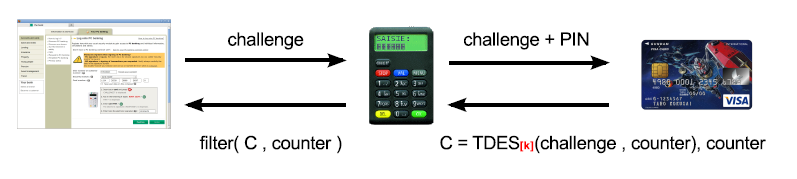
\includegraphics[scale=0.6]{img/mode1-ebanking}
	\end{center}
	
\item Mode 2 (insecure): Signature of a financial transaction
	\begin{center}
		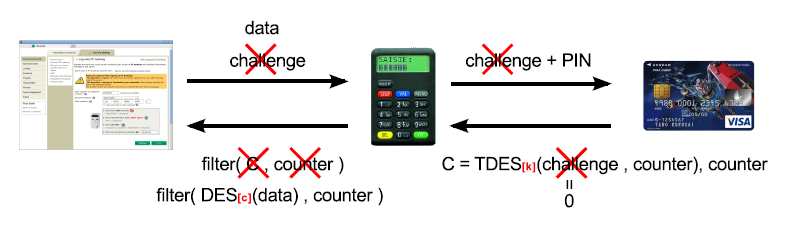
\includegraphics[scale=0.6]{img/mode2-ebanking}
	\end{center}
\end{itemize}
The first mode is secure but with the second replay attack is possible. %preplay too?


\subsection{Digital Signature Transponder}


Texas Instruments Digital Signature Transponder is a tag used to enable 
fuel-injection system of the vehicle.
\begin{itemize}
	\item It uses a Proprietary cipher that uses 40-bit keys
	\item DST responses to 8 queries per second.
\end{itemize}

\subsubsection{Authentication protocol}
\begin{tabular}{m{8cm}m{8cm}}
    \begin{tabular}{ccc}
        \bf Verifier & &\bf  Prover \\
                 &\fr{r} & \\
        \\
        & \fl{id, $Trunc_{24}(E_k(r))$, checksum} \\
    \end{tabular}
    &
    \begin{itemize}
        \item |k| = |r| = |$E_k(r)$| = 40bits
        \item |identifier| = |$Truncate_{24}(E_k(r))$| = 24 bits
        \item |checksum| = 16 bits
    \end{itemize}
\end{tabular}

\subsubsection{Brute force attacks}
An attack has been performed on this system which consist of:
\begin{enumerate}
    \item Reverse engineering the cipher (because they use a proprietary
        encryption)
	\item Eavesdropping some communications\footnote{One communication is
    sufficient if no truncation as the truncation is a mapping N to 1}
	\item Recovering the key using a brute force attack (feasible as $|k|$ is small)
	\item Simulating the tag to init the targeted tag
\end{enumerate}

\subsubsection{Pigeon holes attacks}
It can occur when we have a truncation, it means that the input set is
greater than the output set.

$$A, B \textrm{ two set s.t  } |A| > |B|, \quad f(A\rightarrow B) \quad
\Rightarrow \exists x, y \in A: f(x) = f(y)$$

\begin{tabular}{m{7cm}m{8cm}}
    \centering
    \begin{tikzpicture}[node distance=0.3cm]
    \node[draw, circle, fill=red] (H1) {};
    \node[draw, circle, right=of H1] (H2) {};
    \node[draw, circle, right=of H2] (H3) {};
    \node[draw, circle, right=of H3] (H4) {};

    \node[draw, rectangle, below=1cm of H1] (P3) {};
    \node[draw, rectangle, left=of P3, fill=red] (P1) {};
    \node[draw, rectangle, left=of P3] (P2) {};
    \node[draw, rectangle, right=of P3] (P4) {};
    \node[draw, rectangle, right=of P4] (P5) {};
    \node[draw, rectangle, right=of P5] (P6) {};
    \node[draw, rectangle, right=of P6] (P7) {};
    \node[draw, rectangle, right=of P7] (P8) {};

    \node[draw, rectangle, rounded corners=2pt, fit={(P1) (P8)}] (F) {};
    \node[draw, rectangle, rounded corners=2pt, fit={(H1) (H4)}] (FF) {};

    \node[left=of F] {B};
    \node[left=of FF] {A};

    \draw (P1) edge[->] (H1);
    \end{tikzpicture}
    &
            Probability to uniquely identified a pigeon:
            $$P = \big(\frac{B\textcolor{red}{-1}}{B}\big)^{A\textcolor{red}{-1}}$$

\end{tabular}


\paragraph{Attacks}
The goal is to identify the key:
\begin{enumerate}
    \item Pre-compute a table for a fixed random $r$: 
        \begin{tabular}{cc|c}
            &Key & Result   \\
            \hline
            \multirow{3}{*}{\rotatebox{90}{All keys}} &
            $k_1$ & $Trunc_{24}(E_{k_1}(r))$\\
                  & $\vdots$ & $\vdots$ \\
                  & $k_{2^{40}}$ & $Trunc_{24}(E_{k_{2^{40}}}(r))$\\

            \end{tabular}

        \item After send a random $r$, we have a probability to uniquely
            identified the correct key:
            $$P = \big(\frac{2^{24}-1}{2^{24}}\big)^{2^{40}-1} \approx 0$$

        \item We recompute a table for a other random number $r'$ and
            resend this number. Now, he have a probability to uniquely
            identified the correct key:
            $$P = \big(\frac{2^{24}-1}{2^{24}}\big)^{2^{16}-1} \approx
            0.996$$

            Note that we have now $2^{16}$ which is the maximum number
            of key such that $E_k(r)$ are different but
            $Trunc_{24}(E_k(r))$ is the same.
\end{enumerate}

\subsubsection{Security}
\begin{itemize}
	\item Because the tag respond to any challenge, it's possible to challenge it instead
	of eavesdropping it
	\item Since the tag response is truncated, using a brute force on one 
	challenge/response pair leads to several possible keys ( pigeonhole principle)
	\item Authors managed to recover a key with 16 FGPAs in parallel
\end{itemize}


